% Created 2015-03-21 Sat 10:22
\documentclass[11pt]{article}
\usepackage[utf8]{inputenc}
\usepackage[T1]{fontenc}
\usepackage{fixltx2e}
\usepackage{graphicx}
\usepackage{longtable}
\usepackage{float}
\usepackage{wrapfig}
\usepackage{rotating}
\usepackage[normalem]{ulem}
\usepackage{amsmath}
\usepackage{textcomp}
\usepackage{marvosym}
\usepackage{wasysym}
\usepackage{amssymb}
\usepackage{hyperref}
\tolerance=1000
\author{世凡 黄}
\date{\today}
\title{2015年“得食乐Fun享”微信游戏实现方案}
\hypersetup{
  pdfkeywords={},
  pdfsubject={},
  pdfcreator={Emacs 24.4.1 (Org mode 8.2.10)}}
\begin{document}

\maketitle
\tableofcontents


\section{概述}
\label{sec-1}
\subsection{简介}
\label{sec-1-1}
基于微信公众平台的得分赢礼卷游戏。
\begin{itemize}
\item 该活动每位用户仅限 \textbf{一张} 赢取礼卷的机会(分数达 \textbf{320分} 以上);
\item 排行前3的活动结束将有机会获取最终大奖,将有专人联系你(最终解析权为主办方)
\item 礼卷使用方式,用微信二维码扫礼卷中得二维码会得知该卷是否使用过,
主要扫过一次就代表该卷已使用(如下展示扫码结果,扫描成功后将跳转网页。
如下效果不是最终展示效果,效果以具体最终实现为准)

\includegraphics[width=.9\linewidth]{imgs/coupon.jpg}
\end{itemize}

游戏前端功能如下:
\begin{itemize}
\item 游戏主体逻辑(以点击消除物品来获取分值)
\item 获取微信用户资料(头像,昵称等)
\item 礼卷(只获取,在用户分数到达 \textbf{320} 分,且每个用户仅限获取一张)
\item 查看游戏积分排行榜(前 \textbf{十} 位)
\end{itemize}


公众号功能如下:
\begin{itemize}
\item 活动菜单(二级菜单,名为“得食乐Fun享”),
点击触发多图文消息(1.进入游戏,2.查看礼卷)
\item 获取当前用户资料,在开始游戏时,通过页面赋值(查看\hyperref[user_login]{用户模块\#用户登陆授权})
\item 礼卷录入(具体信息请看\hyperref[coupon]{礼卷模块})
\item 礼卷生成(主要涉及到二维码生成,详阅\hyperref[coupon]{礼卷模块})
\item 礼卷使用(标记该礼卷已使用,与生成得二维码相关,详阅\hyperref[coupon]{礼卷模块})
\item 用户最高分值记录并排行(详阅\hyperref[user_score_submit]{用户模块\#上传积分})
\item 返回排行数据(前 \textbf{十} 名)
\end{itemize}

\subsection{流程}
\label{sec-1-2}

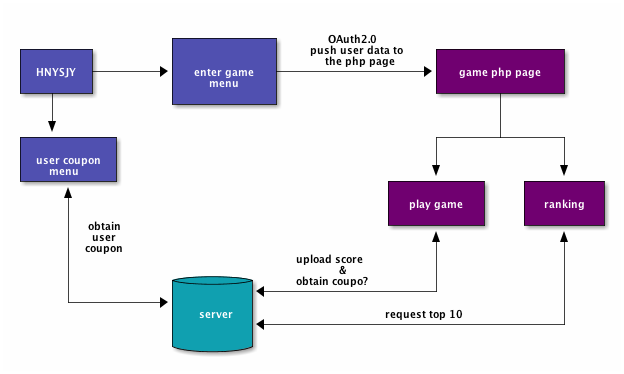
\includegraphics[width=.9\linewidth]{imgs/flowchart.png}

说明
\begin{center}
\begin{tabular}{ll}
描述 & 作用\\
\hline
蓝色 & 微信客户端(主办方公众号)\\
紫色 & 游戏前端\\
青色 & 公众号服务端\\
HNYSJY & 微信公众号\\
\end{tabular}
\end{center}


\section{用户模块\label{user}}
\label{sec-2}
\subsection{用户登陆授权\label{user_login}}
\label{sec-2-1}

\subsubsection{描述}
\label{sec-2-1-1}
通过OAuth2.0获取换取到用户信息,服务器端渲染游戏页面perish-game.php,流程如下:
\begin{enumerate}
\item 微信公众账号提供用户请求授权页面URL
\item 用户点击授权页面URL,将向服务器发起请求
\item 服务器询问用户是否同意授权给微信公众账号
\item 服务器将code通过回调传给微信公众账号
\item 微信公众账号通过CODE向服务器请求access$_{\text{token}}$
\item 微信公众账号通过access$_{\text{oken向服务器请求用户信息}}$
\item 利用用户信息渲染perish-game.php并返回给用户
\end{enumerate}



\subsection{上传积分\label{user_score_submit}}
\label{sec-2-2}

\section{礼卷模块\label{coupon}}
\label{sec-3}



\section{\textbf{TODO}}
\label{sec-4}
% Emacs 24.4.1 (Org mode 8.2.10)
\end{document}
